\chapter{Detalhes da Implementação}

\section{Introdução}

Este capítulo detalha a implementação do sistema de treinamento e inserção automática desenvolvido para a geração de ambientes virtuais a partir de imagens. A aplicação foi concebida para automatizar o processo de geração de modelos tridimensionais a partir das imagens processadas. O objetivo principal da implementação é oferecer uma solução eficiente para qualquer usuário que deseja criar ambientes virtuais, possa fazê-lo de maneira rápida e intuitiva, com base em imagens fornecidas.

A aplicação, desenvolvida dentro da plataforma Unity, permite ao usuário carregar imagens através de um menu gráfico e, a partir delas, o sistema realiza automaticamente o reconhecimento dos objetos presentes dentro da foto fornecida e os insere no ambiente virtual. Essa abordagem reduz significativamente a necessidade de intervenção manual, tornando o processo de criação de ambientes 3D mais eficiente. A automação deste processo é particularmente útil para usuários com pouca experiência técnica na geração de ambientes virtuais, permitindo-lhes focar na interatividade do ambiente ambiente sem se preocupar com os detalhes gráficos.


\subsection{Estrutura geral da aplicação}

A estrutura da aplicação desenvolvida neste trabalho está representada na Figura \ref{fig:estrutura}. A arquitetura do sistema é composta por quatro elementos principais que operam em conjunto para realizar a tarefa de criação de ambientes virtuais. O fluxo do processo inicia-se com o treinamento do modelo YOLO, que gera os pesos da RNC utilizados no reconhecimento de objetos nas imagens fornecidas.

\begin{figure}[!h]
    \centering
    \begin{minipage}{1\linewidth}
    \centering
    \captionsetup{justification=centering,margin=0.5cm,font=small}
    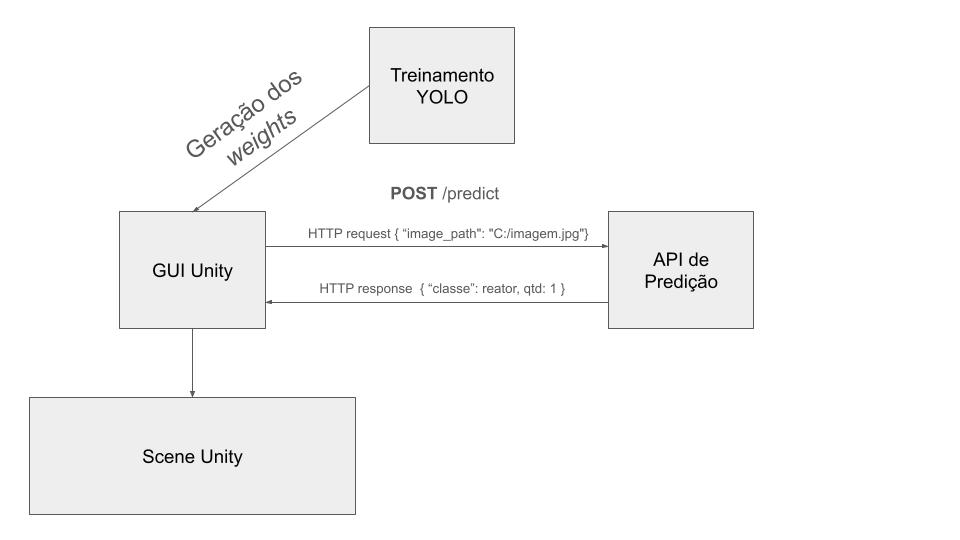
\includegraphics[width=1\linewidth]{img/cap5/estrutura.jpg}
    \caption{Estrutura geral da Aplicação}.
    \label{fig:estrutura}
    \end{minipage}
\end{figure}

O segundo componente importante da estrutura é a interface gráfica do usuário (\textit{Graphical User Interface} - GUI) no Unity, que pode ser visualizada na Figura \ref{fig:GUI}. Esta interface foi cuidadosamente projetada para facilitar a identificação e modelagem das cenas virtuais. O script que compõe a GUI é integrado diretamente ao Unity, proporcionando ao usuário uma ferramenta intuitiva para selecionar imagens e iniciar o processo de reconhecimento. A GUI comunica-se com uma \textit{API} que aplica o modelo treinado às imagens fornecidas, enviando uma requisição \textit{HTTP} com os dados necessários

Conforme ilustrado no diagrama, a \textit{API} recebe o caminho da imagem, aplica os pesos treinados da RNC, e retorna ao Unity a quantidade de objetos identificados e suas respectivas classes. No caso, o protótipo foi desenvolvido para trabalhar com apenas uma classe, abrindo espaço para trabalhos futuros, assim como ele também não implementa a localização espacial dos objetos, os modelos virtuais gerados são dispostos de forma uniforme na cena do Unity após o processamento da imagem. Isso significa que, apesar da precisão na detecção dos objetos, ainda há espaço para melhorias no que diz respeito à colocação exata dos modelos dentro do ambiente virtual, o que será uma possível melhoria em versões futuras do sistema.

\begin{figure}[!h]
    \centering
    \begin{minipage}{0.7\linewidth}
        \centering
        \captionsetup{justification=centering,margin=0.5cm,font=small}
        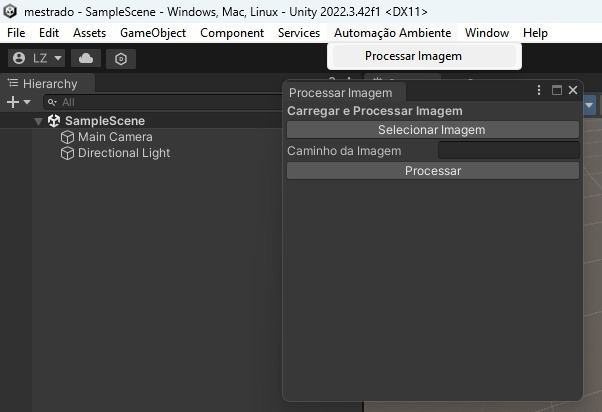
\includegraphics[width=\linewidth]{img/cap5/GUI-TOOL.jpeg}
        \caption{Interface para o usuário.}
        \label{fig:GUI}
    \end{minipage}
\end{figure}

\subsection{Treinamento com a YOLO}

O treinamento com o YOLO segue um padrão comum entre suas diferentes versões, mas cada versão possui características específicas em termos de pacotes necessários e processos de instalação. A estrutura básica do script de treinamento da YOLOv8 inclui a importação dos pacotes necessários para o funcionamento do modelo, geralmente nas primeiras linhas do arquivo. Em seguida, a escolha da arquitetura de treinamento, neste caso ‘yolov8n.pt’, e por fim, a linha responsável pela execução do treinamento, que recebe como parâmetros as características da rede neural, como a quantidade de épocas, o tipo de otimizador, entre outros (Figura \ref{fig:script-yolov8}). A flexibilidade do treinamento permite ajustar o modelo para obter o melhor desempenho possível de acordo com as necessidades específicas do usuário, sendo possível a customização de diversos parâmetros.

\begin{figure}[!h]
    \centering
    \begin{minipage}{0.7\linewidth}
    \centering
    \captionsetup{justification=centering,margin=0.5cm,font=small}
    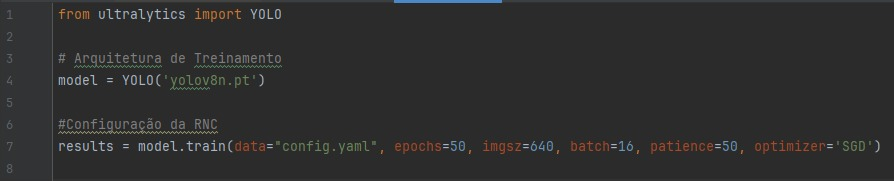
\includegraphics[width=1\linewidth]{img/cap5/treinamentoYOLOv8.jpeg}
    \caption{Demonstração do Script de Treinamento da YOLOv8}.
    \label{fig:script-yolov8}
    \end{minipage}
\end{figure}

\subsection{API de Identificação}

A construção da aplicação responsável pelo processamento das imagens enviadas pelo Unity envolveu a criação de um \textit{endpoint} que permite a solicitação do serviço de processamento por aplicações externas. O Unity envia uma requisição \textit{HTTP} para o endereço \textit{"localhost:5000/predict"}, incluindo o caminho da imagem no corpo da requisição. Ao receber a requisição, o \textit{endpoint} aplica a função de predição, existente dentro dos pacotes da YOLO, e processa a imagem. Em seguida, o sistema percorre os resultados da predição e extrai as informações relevantes, como a quantidade de reatores identificados.

\begin{figure}[!h]
    \centering
    \begin{minipage}{0.7\linewidth}
    \centering
    \captionsetup{justification=centering,margin=0.5cm,font=small}
    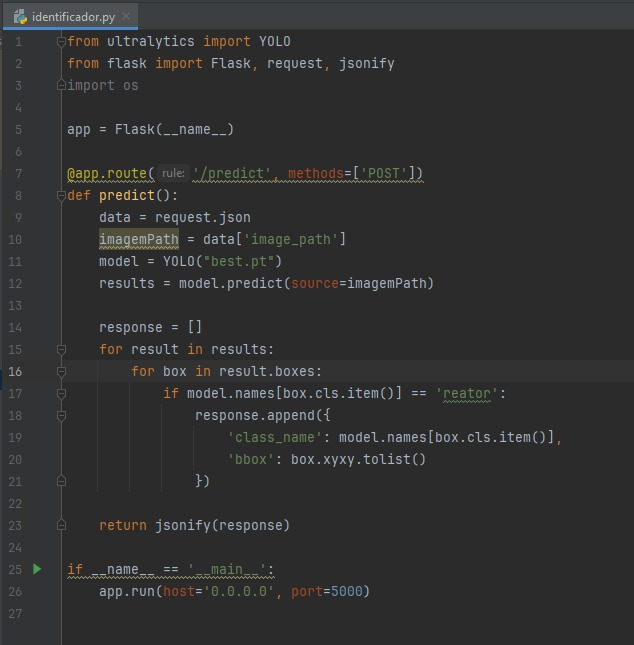
\includegraphics[width=1\linewidth]{img/cap5/API.jpeg}
    \caption{\textit{API} de identificação de imagem}.
    \label{fig:script-yolov8}
    \end{minipage}
\end{figure}

Para executar esta aplicação, você precisará do Python 3.5 ou superior instalado em seu sistema. Pode-se instalar as dependências manualmente usando o comando \textit{pip install}, especificando os pacotes necessários. Neste caso, como o script utiliza Flask e o YOLO da biblioteca Ultralytics, pode-se instalar essas bibliotecas com o seguinte comando: \textit{pip install flask ultralytics}. Após instalar as dependências, supondo que o script seja salvo em um arquivo chamado \textit{api-rv.py}, abra um terminal no diretório onde o script está localizado e execute o comando: \textit{python api-rv.py}. Isso iniciará o servidor Flask e tornará o endpoint \textit{"/predict"} acessível para aplicações externas, como o Unity. O código completo do script \textit{api-rv.py} está localizado no Apêndice A.

\subsection{Implementação no Unity}

O script desenvolvido no Unity é dividido em alguns métodos. Inicialmente, há a disposição na tela da interface gráfica, representada na Figura \ref{fig:metodo-gui}. Este código define o nome da janela, suas dimensões e os tipos de interações que o usuário pode realizar, como selecionar uma imagem e iniciar o processamento. A GUI foi desenvolvida com foco na usabilidade, garantindo que até mesmo usuários com pouca experiência em Unity possam operar a implementação com facilidade. O código completo que habilita esta implementação dentro do Unity, entitulado \textit{ModelLoaderMenu.cs}, está localizado no Apêndice B. Copiá-lo em um arquivo homônimo e colocá-lo dentro do projeto Unity é suficiente para poder utilizá-lo.

\begin{figure}[!h]
    \centering
    \begin{minipage}{0.7\linewidth}
    \centering
    \captionsetup{justification=centering,margin=0.5cm,font=small}
    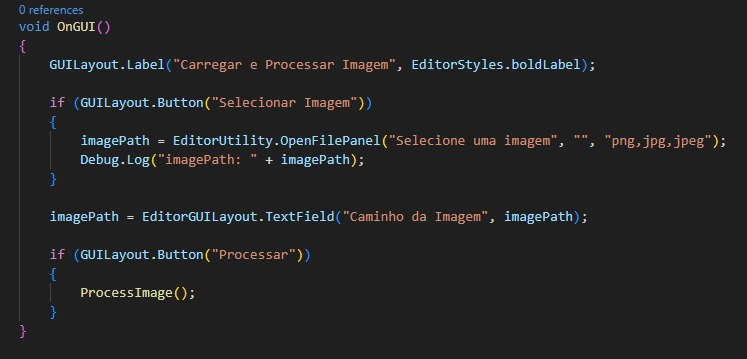
\includegraphics[width=1\linewidth]{img/cap5/gui-codigo.jpeg}
    \caption{\textit{API} de identificação de imagem}.
    \label{fig:metodo-gui}
    \end{minipage}
\end{figure}

Ao pressionar o botão de processamento, o método correspondente é ativado, conforme ilustrado na Figura \ref{fig:metodo-disposicao}. Este método chama outro, que é responsável por enviar a requisição \textit{HTT} para a \textit{API} processar a resposta recebida. Com as informações retornadas pela \textit{API}, o \textit{script} percorre cada objeto identificado e o insere na cena do Unity, posicionando-os de acordo com uma disposição pré-definida. Embora o sistema ainda não implemente uma disposição espacial precisa dos objetos, ele serve como uma base sólida para futuras melhorias.

\begin{figure}[!h]
    \centering
    \begin{minipage}{0.7\linewidth}
    \centering
    \captionsetup{justification=centering,margin=0.5cm,font=small}
    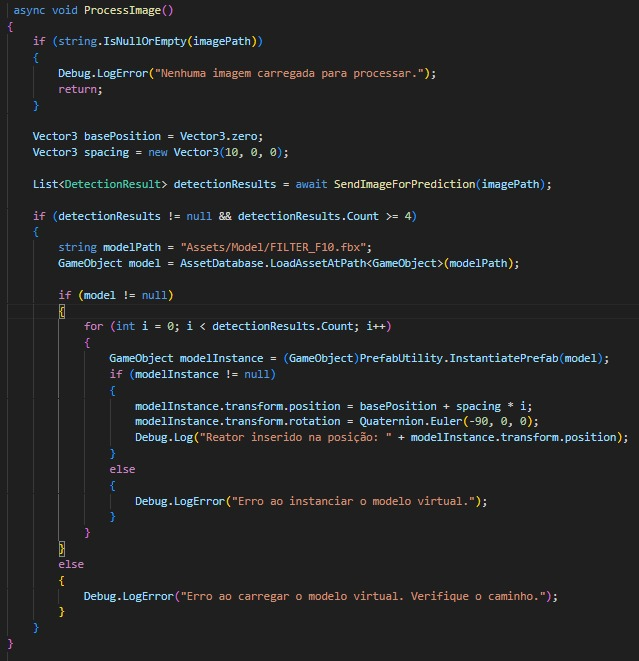
\includegraphics[width=1\linewidth]{img/cap5/process-image.jpeg}
    \caption{Método de processamento da imagem e inserção dos modelos conforme a resposta da \textit{API}}.
    \label{fig:metodo-disposicao}
    \end{minipage}
\end{figure}

Após o processamento da imagem, o número de reatores identificados pelo modelo é automaticamente renderizado na cena do Unity. Essa etapa garante que os objetos reconhecidos sejam visualmente representados no ambiente virtual, facilitando a interação e análise do usuário. A Figura \ref{fig:predict} ilustra um exemplo de imagem processada, na qual foram corretamente identificados e inseridos quatro reatores na cena. A quantidade de reatores e outros objetos detectados e inseridos na cena depende diretamente da precisão do modelo de reconhecimento utilizado, bem como da qualidade e clareza dos elementos presentes na imagem original. Dessa forma, um modelo bem treinado, aliado a uma imagem nítida e bem enquadrada, resulta em uma identificação mais precisa e uma correspondência fiel entre os objetos detectados e os inseridos no ambiente virtual. Esse processo automatizado não apenas melhora a eficiência da criação de cenas no Unity, mas também minimiza a necessidade de ajustes manuais, proporcionando uma experiência mais fluida e prática para o usuário.

\begin{figure}[!h]
    \centering
    \begin{minipage}{0.9\linewidth}
    \centering
    \captionsetup{justification=centering,margin=0.5cm,font=small}
    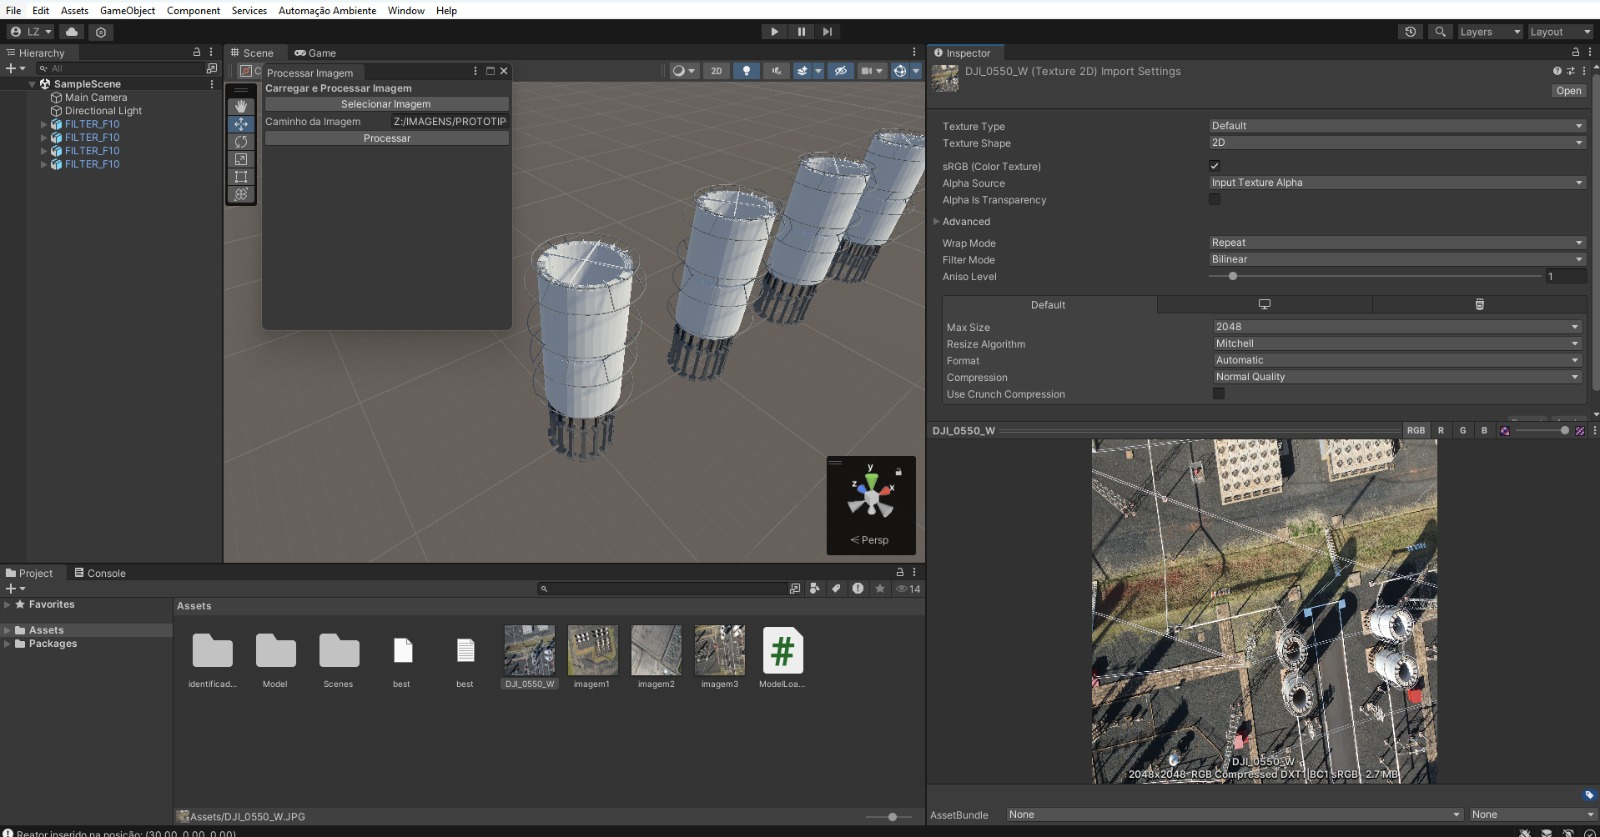
\includegraphics[width=1\linewidth]{img/cap5/predict.jpeg}
    \caption{Método de processamento da imagem e inserção dos modelos conforme a resposta da \textit{API}}.
    \label{fig:predict}
    \end{minipage}
\end{figure}

\subsection{Conclusão}

A implementação desenvolvida é altamente intuitiva e de fácil utilização. Para executá-la em um computador pessoal, basta inserir o script direcionado para o Unity dentro do projeto e, em paralelo, rodar o código da \textit{API} em um arquivo separado. Essa aplicação se destaca como uma solução prática e eficiente, oferecendo um método simplificado que pode gerar um impacto significativo no desenvolvimento de ambientes de RV.


	





